%%%%%%%%%%%%%%%%%%%%%%%%%%%%%%%%%%%%%%%%%
% Short Sectioned Assignment
% LaTeX Template
% Version 1.0 (5/5/12)
%
% This template has been downloaded from:
% http://www.LaTeXTemplates.com
%
% Original author:
% Frits Wenneker (http://www.howtotex.com)
%
% License:
% CC BY-NC-SA 3.0 (http://creativecommons.org/licenses/by-nc-sa/3.0/)
%
%%%%%%%%%%%%%%%%%%%%%%%%%%%%%%%%%%%%%%%%%

%----------------------------------------------------------------------------------------
%	PACKAGES AND OTHER DOCUMENT CONFIGURATIONS
%----------------------------------------------------------------------------------------

\documentclass[paper=a4, fontsize=11pt]{scrartcl} % A4 paper and 11pt font size

\usepackage[T1]{fontenc} % Use 8-bit encoding that has 256 glyphs
%\usepackage{fourier} % Use the Adobe Utopia font for the document - comment this line to return to the LaTeX default
\usepackage[english]{babel} % English language/hyphenation
\usepackage{amsmath,amsfonts,amsthm} % Math packages

\usepackage{sectsty} % Allows customizing section commands
%\allsectionsfont{\centering \normalfont\scshape} % Make all sections centered, the default font and small caps
\allsectionsfont{\centering}

\usepackage{fancyhdr} % Custom headers and footers
\pagestyle{fancyplain} % Makes all pages in the document conform to the custom headers and footers
\fancyhead{} % No page header - if you want one, create it in the same way as the footers below
\fancyfoot[L]{} % Empty left footer
\fancyfoot[C]{} % Empty center footer
\fancyfoot[R]{\thepage} % Page numbering for right footer
\renewcommand{\headrulewidth}{0pt} % Remove header underlines
\renewcommand{\footrulewidth}{0pt} % Remove footer underlines
\setlength{\headheight}{13.6pt} % Customize the height of the header

%\numberwithin{equation}{section} % Number equations within sections (i.e. 1.1, 1.2, 2.1, 2.2 instead of 1, 2, 3, 4)
%\numberwithin{figure}{section} % Number figures within sections (i.e. 1.1, 1.2, 2.1, 2.2 instead of 1, 2, 3, 4)
%\numberwithin{table}{section} % Number tables within sections (i.e. 1.1, 1.2, 2.1, 2.2 instead of 1, 2, 3, 4)

%\setlength\parindent{0pt} % Removes all indentation from paragraphs - comment this line for an assignment with lots of text

\theoremstyle{plain}
\newtheorem{lemma}{Lemma}

%\usepackage{caption}
\usepackage{topcapt}
\usepackage{booktabs}

\usepackage{float}
\restylefloat{table}

\usepackage{graphicx}
\graphicspath{{../images/}}



%----------------------------------------------------------------------------------------
%	TITLE SECTION
%----------------------------------------------------------------------------------------

\newcommand{\horrule}[1]{\rule{\linewidth}{#1}} % Create horizontal rule command with 1 argument of height

\title{	
\normalfont \normalsize 
\textsc{UPC - Complex and Social Networks} \\ [25pt] % Your university, school and/or department name(s)
\horrule{0.5pt} \\[0.4cm] % Thin top horizontal rule
\huge Lab 2: Analysis of the degree distribution\\ % The assignment title
\horrule{2pt} \\[0.5cm] % Thick bottom horizontal rule
}

\author{Michele Gentili and Simon Van den Eynde} % Your name

\date{\normalsize\today} % Today's date or a custom date

\begin{document}

\maketitle % Print the title


%----------------------------------------------------------------------------------------
%	INTRO
%----------------------------------------------------------------------------------------
\section{Introduction}
In this lab we will try to select a theoretic model, fitting the degree distribution of syntactic dependency networks in different languages. We will focus on in-degrees.

We considered $5$ theoretical models and used the Akaike information criterions (AIC) to decide which model was most favourable. The models we considered were
\begin{enumerate}
\item a zeta distribution
\item a zeta distribution with fixed exponent $2$
\item a right-truncated zeta distribution
\item a geometric distribution 
\item a geometric displaced distribution  
\item a displaced poisson distribution
\end{enumerate}

After choosing the statistically best models, we plotted our models to our data to do a visual check of correctness.

And finally recompute the Akaike scores, introducing a better model: the Altmann distribution.

%----------------------------------------------------------------------------------------
%	RESULTS
%----------------------------------------------------------------------------------------
\section{Results}

In table~\ref{diffAIC} we find our main result, the difference in AIC from the best (of the $5$) model. We notice that except for Hungarian and Turkish the right-truncated zeta always ends up best.\\

% latex table generated in R 3.1.2 by xtable 1.7-4 package
% Wed Oct 12 18:23:23 2016
\begin{table}[h!!!]
\centering
\topcaption{Difference in AIC for the $5$ different models in different languages} \label{diffAIC}
\begin{tabular}{rrrrrr}
 &&&Models&&\\
  \hline
 Language & 1 & 2 & 3 & 4 & 5 \\ 
  \hline
Arabic & 2.91 & 175.28 & 0.00 & 24188.95 & 240321.25 \\ 
  Basque & 0.24 & 845.41 & 0.00 & 8364.11 & 50164.59 \\ 
  Catalan & 13.96 & 225.90 & 0.00 & 61881.73 & 913880.09 \\ 
  Chinese & 14.69 & 503.99 & 0.00 & 48678.82 & 618348.40 \\ 
  Czech & 8.85 & 147.28 & 0.00 & 91099.39 & 940677.71 \\ 
  English & 45.05 & 1469.66 & 0.00 & 45742.18 & 739581.47 \\ 
  Greek & 3.43 & 164.11 & 0.00 & 17133.83 & 157137.24 \\ 
  Hungarian & 0.00 & 2220.28 & 1.71 & 53469.62 & 468252.20 \\ 
  Italian & 0.49 & 118.37 & 0.00 & 22877.90 & 245803.51 \\ 
  Turkish & 0.00 & 2740.47 & 1.98 & 24615.35 & 193345.03 \\ 
   \hline
\end{tabular}
\end{table}

In table~\ref{rss} we find the RSS-values for the zeta and right-truncated zeta distribution. We notice that in both table \ref{diffAIC} and \ref{rss} most values for the zeta and right-truncated zeta are very alike.

% latex table generated in R 3.1.2 by xtable 1.7-4 package
% Wed Oct 12 21:46:55 2016
\begin{table}[ht]
\centering
\topcaption{RSS values for zeta and right-truncated zeta distribution with optimised parameters}\label{rss}
\begin{tabular}{rrr}
  \hline
 & zeta & RT\_zeta \\ 
  \hline
Arabic & 9.54e-04 & 9.33e-04 \\ 
  Basque & 1.68e-05 & 1.78e-05 \\ 
  Catalan & 1.12e-04 & 1.03e-04 \\ 
  Chinese & 5.21e-04 & 4.94e-04 \\ 
  Czech & 4.12e-05 & 3.82e-05 \\ 
  English & 3.46e-04 & 2.90e-04 \\ 
  Greek & 4.38e-04 & 4.15e-04 \\ 
  Hungarian & 3.93e-04 & 3.94e-04 \\ 
  Italian & 1.82e-04 & 1.75e-04 \\ 
  Turkish & 6.92e-05 & 6.92e-05 \\ 
   \hline
\end{tabular}
\end{table}

% latex table generated in R 3.3.1 by xtable 1.8-2 package
% Thu Oct 13 19:43:22 2016
In table~\ref{diffAIC_A} we added two more models, the Altmann model and a corrected geometric model (see also Method section). As we expected has the Altmann function best score, so all the other values are shifted of the difference between the previous best model score and the Altmann score.

% latex table generated in R 3.1.2 by xtable 1.7-4 package
% Thu Oct 13 23:20:49 2016
\begin{table}[H]
\centering
\topcaption{Difference in AIC for the $5$ different models + 2 extra models in different languages} \label{diffAIC_A}
\begin{tabular}{rrrrrrrr}
  \hline
 & zeta & zeta\_2 & RT\_zeta & geom & poisson & geom\_corrected & Altmann \\ 
  \hline
Arabic & 132092 & 132264 & 132089 & 156278 & 372410 & 137774 &   0 \\ 
  Basque & 58151 & 58996 & 58151 & 66515 & 108315 & 42796 &   0 \\ 
  Catalan & 271389 & 271601 & 271375 & 333256 & 1185255 & 318171 &   0 \\ 
  Chinese & 277583 & 278072 & 277568 & 326247 & 895917 & 309159 &   0 \\ 
  Czech & 439807 & 439946 & 439799 & 530898 & 1380476 & 485598 &   0 \\ 
  English & 251394 & 252819 & 251349 & 297091 & 990930 & 287081 &   0 \\ 
  Greek & 78708 & 78869 & 78705 & 95839 & 235842 & 85490 &   0 \\ 
  Hungarian & 185034 & 187254 & 185036 & 238504 & 653286 & 204135 &   0 \\ 
  Italian & 86617 & 86735 & 86617 & 109495 & 332420 & 101040 &   0 \\ 
  Turkish & 91486 & 94227 & 91488 & 116101 & 284831 & 80961 &   0 \\ 
   \hline
\end{tabular}
\end{table}

Hereafter we added a plot for every language, plotting the fit of some distributions on the data.


%Example Image
\begin{figure}[!htbp] %  figure placement: here, top, bottom, or page
   \centering
   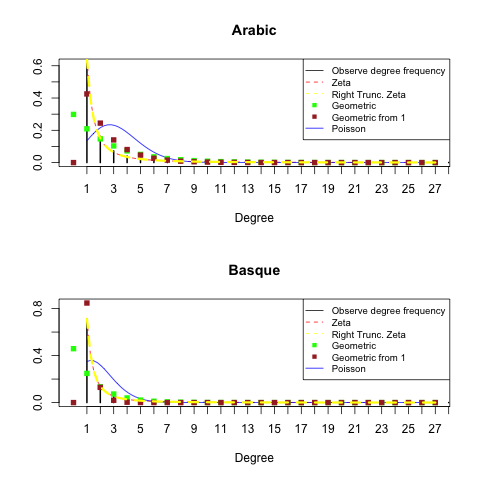
\includegraphics[width=\textwidth]{General_1} %width can also be 2in, 3.5in, .5\textwidth?
  
\end{figure}

%Example Image
\begin{figure}[htbp] %  figure placement: here, top, bottom, or page
   \centering
   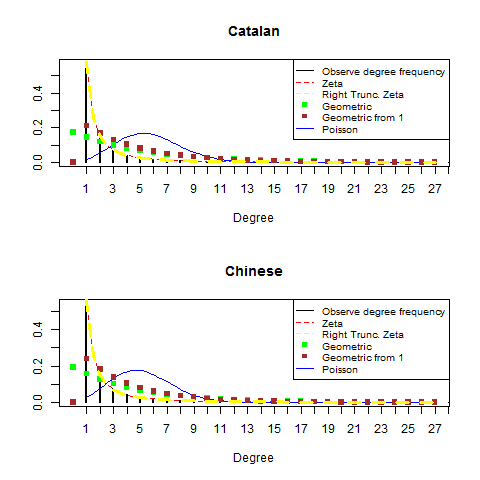
\includegraphics[width=\textwidth]{General_2} %width can also be 2in, 3.5in, .5\textwidth?

\end{figure}

%Example Image
\begin{figure}[htbp] %  figure placement: here, top, bottom, or page
   \centering
   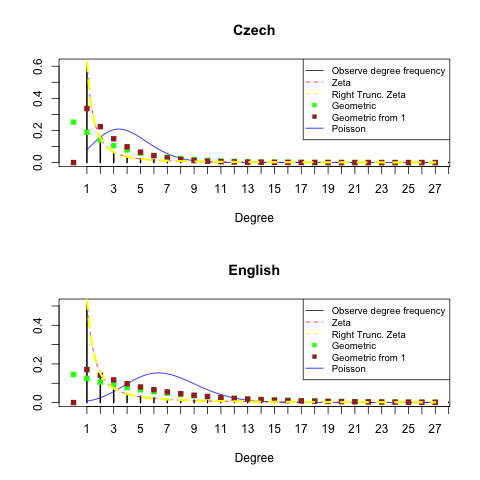
\includegraphics[width=\textwidth]{General_3} %width can also be 2in, 3.5in, .5\textwidth?
\end{figure}

%Example Image
\begin{figure}[htbp] %  figure placement: here, top, bottom, or page
   \centering
   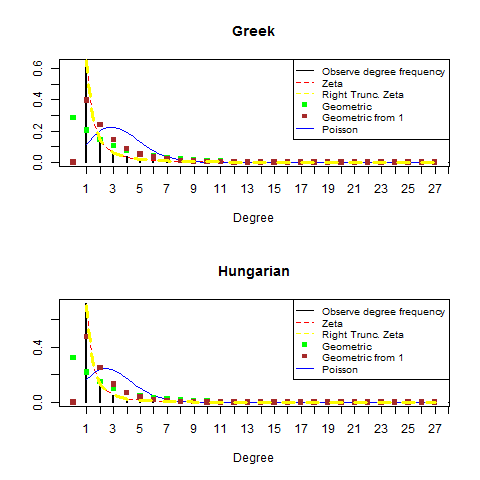
\includegraphics[width=\textwidth]{General_4} %width can also be 2in, 3.5in, .5\textwidth?
\end{figure}

%Example Image
\begin{figure}[htbp] %  figure placement: here, top, bottom, or page
   \centering
   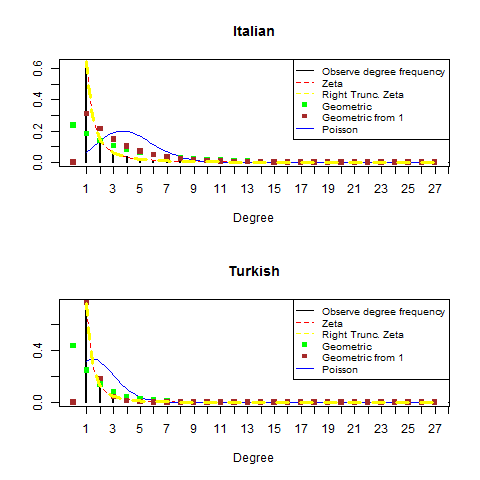
\includegraphics[width=\textwidth]{General_5} %width can also be 2in, 3.5in, .5\textwidth?
\end{figure}

And we also added some extra plots regarding the Altmann distribution.

%Example Image
\begin{figure}[htbp] %  figure placement: here, top, bottom, or page
   \centering
   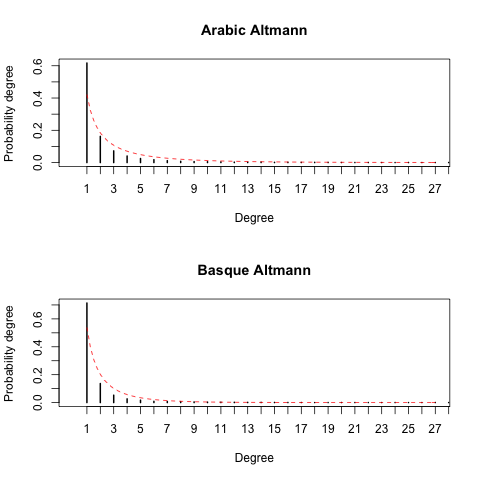
\includegraphics[width=\textwidth]{Altman_1} %width can also be 2in, 3.5in, .5\textwidth?
\end{figure}

%Example Image
\begin{figure}[htbp] %  figure placement: here, top, bottom, or page
   \centering
   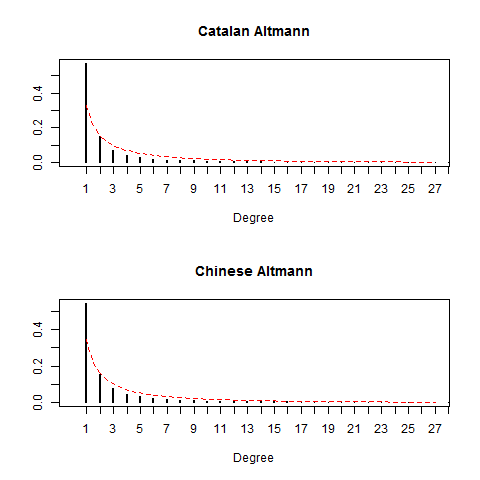
\includegraphics[width=\textwidth]{Altman_2} %width can also be 2in, 3.5in, .5\textwidth?
\end{figure}

%Example Image
\begin{figure}[htbp] %  figure placement: here, top, bottom, or page
   \centering
   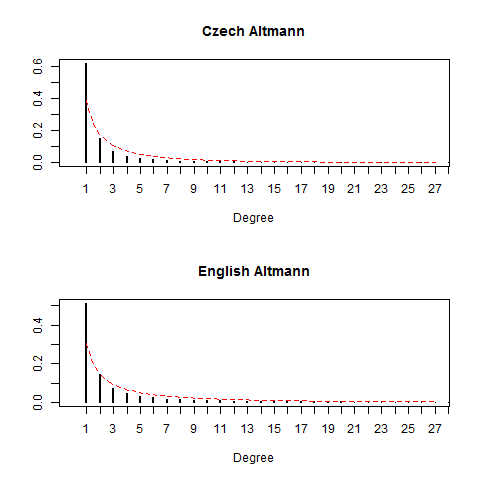
\includegraphics[width=\textwidth]{Altman_3} %width can also be 2in, 3.5in, .5\textwidth?
\end{figure}

%Example Image
\begin{figure}[htbp] %  figure placement: here, top, bottom, or page
   \centering
   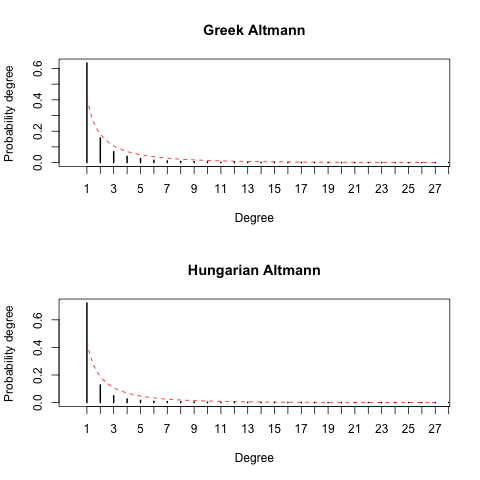
\includegraphics[width=\textwidth]{Altman_4} %width can also be 2in, 3.5in, .5\textwidth?
   \label{fig:example}
\end{figure}

%Example Image
\begin{figure}[htbp] %  figure placement: here, top, bottom, or page
   \centering
   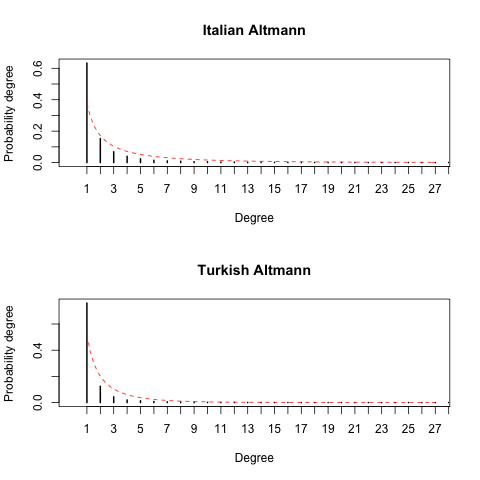
\includegraphics[width=\textwidth]{Altman_5} %width can also be 2in, 3.5in, .5\textwidth?
   \caption{example caption}
   \label{fig:example}
\end{figure}




\newpage

%----------------------------------------------------------------------------------------
%	DISCUSSION
%----------------------------------------------------------------------------------------
\section{Discussion}
When optimising model $3$ we noticed that the value of $k_{max}$ stays its starting value and does not change, while manually changing the starting value of $k_{max}$ and thus the value obtained by optimising, significantly improved the AIC-value and the RSS-value. For the english-in-degree-sequence reduces changing $k_{max}$ manually from max degree to $778$ the RSS by over $30\%$.

On the plots we see that the Altmann distribution and the (right-truncated)-zeta distribution fit the probabilities from the data well. We prefer the Altmann distribution over the the zeta-distributions because the Altmann distribution has a lower AIC.

\subsection{Conclusion}
The best model is the Altmann model, the zeta function with respect to the previous functions works better because it behaves good on the tails, the geometric distribution, even if shifted to 1, 'loses' too much probability on the tails.
Finally as was expected, the difference in AIC has changed as soon as you introduce a better model.\\

Because the Altmann distribution also gives a reasonable fit on the plot, we think that using the altmann distribution is an appropriate way to model the data.

%----------------------------------------------------------------------------------------
%	METHODS
%----------------------------------------------------------------------------------------
\section{Methods}
When using the ``L-BFGS-B'' optimisation method for the right truncated zeta model (model $3$), we often encountered errors. We decided to change the optimisation method to the conjugate gradients method ``CG''. Here we couldn't set any lower bound, but that didn't seem to give any problem for our data.\\

We noticed our geometric distribution gave a weight to the value $0$. So we decided to make a corrected geometric distribution, by shifting the data for this distribution by $1$. We called this distribution geom\_corrected.\\

Calculating the mle-function for the Altmann distribution didn't really work out either. So we calculated the optimised parameters 'manually' with the optim-function, which is used inside the mle-function.
























\end{document}